\documentclass{pre-tfg}

\usepackage{listings}
\usepackage{formular}
\usepackage[pdftex]{graphicx}
\usepackage{hyperref}
\usepackage{todonotes}
\usepackage{amsmath}

\showhelp  % comenta o borra para eliminar ayudas

\title{(TITLE)}
\author{María González Gutiérrez}
\docdate{(MONTH)}{2020}


\DeclareGraphicsExtensions{.pdf,.png,.jpg}

\usepackage{color}
\definecolor{gray97}{gray}{.97}
\definecolor{gray75}{gray}{.75}
\definecolor{gray45}{gray}{.45}

\lstset{ frame=Ltb,
     framerule=0pt,
     aboveskip=0.5cm,
     framextopmargin=3pt,
     framexbottommargin=3pt,
     framexleftmargin=0.4cm,
     framesep=0pt,
     rulesep=.4pt,
     backgroundcolor=\color{gray97},
     rulesepcolor=\color{black},
     %
     stringstyle=\ttfamily,
     showstringspaces = false,
     basicstyle=\small\ttfamily,
     commentstyle=\color{gray45},
     keywordstyle=\bfseries,
     %
     numbers=left,
     numbersep=15pt,
     numberstyle=\tiny,
     numberfirstline = false,
     breaklines=true,
   }

% minimizar fragmentado de listados
\lstnewenvironment{listing}[1][]
   {\lstset{#1}\pagebreak[0]}{\pagebreak[0]}

\lstdefinestyle{consola}
   {basicstyle=\scriptsize\bf\ttfamily,
    backgroundcolor=\color{gray75},
   }

\lstdefinestyle{C}
   {language=C,
   }


\renewcommand*\lstlistingname{Listado}



\begin{document}

\maketitle
\tableofcontents

\newpage


\section{INTRODUCCIÓN Y OBJETIVOS}



\section{FANFICTION, ARCHIVE OF OUR OWN Y RELATOS A UTILIZAR}
Un fanfic (abreviatura de “fanfiction”, “ficción del fan”) es una historia basada en una historia ya existente. Son, en esencia, historias creadas sin ánimo de lucro por los fans de un libro, película o videojuego. 

Hay muchas personas que, al terminar un libro, se quedan con ganas de explorar más a fondo el mundo que el autor ha creado, y esta curiosidad, esta necesidad de saber más sobre la historia, les puede llevar a crear sus propias historias en las que especulan sobre el destino de tal o cuál personaje que la obra original deja ambiguo, o la frustración sobre un final indeseado puede llevar a reescribirlo completamente para que encaje con las expectativas del lector. Otras personas van más allá de cambiar los detalles que no les gustan, sino que llevan a cabo exploraciones exhaustivas de los conflictos, los personajes y sus motivaciones. A estas historias se les llama "fanfiction" (o "fanfic"), y nacen del deseo de explorar temas e ideas que uno siente que faltan en la historia original.

Cuando los fans de una misma obra se reúnen y organizan, se crean comunidades fan llamadas "fandoms", que suelen crear foros donde intercambiar sus impresiones, teorías y, por supuesto, fanfiction y otras formas de arte fan. Algunas teorías acaban popularizándose tanto que el fandom acaba formando, a nivel de comunidad, su propia interpretación de la obra original. Por ejemplo, en Harry Potter, el personaje de Ron Weasly es el mejor amigo del protagonista y es bastante claro que el libro quiere dar el mensaje de que Ron es un buen amigo. Sin embargo, debido a que Ron puede actuar de forma egoísta e insensible, en el fandom de Harry Potter la interpretación dominante es que Ron es en realidad un mal amigo, y muchos escritores de fanfic escriben historias en las que Ron y Harry pelean y dejan de ser amigos, o en las que Ron es directamente un villano.

Éste es sólo uno de las formas de escribir fanfic que hay. Existen muchos fanfics que cambian la historia original de formas mucho más radicales, explorando cómo hubiese sido Star Wars si Luke Skywalker hubiese caído al lado oscuro, o cómo actuarían los personajes de Juego de Tronos si fuesen trabajadores normales en una cafetería de Toronto, por poner algunos ejemplos. El fan convertido en autor puede añadir o quitar a la historia original lo que considere oportuno para contar su propia visión personal.

En resumen, las comunidades fan tienen una interpretación propia de la obra original, que influencian los fanfics que los miembros de dicha comunidad van a escribir y, a su vez, los escritores de fanfic también crean y popularizan interpretaciones que se acaban convirtiendo en dominantes. 



El fanfic cae en una zona gris en términos de derechos de autor, pero suele considerarse “fair use”. A día de hoy, la mayoría de fanfics se publican en sitios web de toda índole, destacando entre ellos \href{archiveofourown.org}{Archive Of Our Own}, que es un archivo open-source y sin ánimo de lucro creado expresamente para alojar obras creadas por fans. Según sus datos de mayo de 2020, tiene más de dos millones de usuarios registrados y más de seis millones de trabajos alojados. En particular elegí descargar los fanfics basados en \textit{Good Omens}, un libro de Terry Pratchett y Neil Gaiman, tanto por la cantidad de relatos existente como por mi familiaridad con esa comunidad.

Además de la cantidad y variedad de relatos que aloja, los motivos por el que elegí extraer los datos de Archive Of Our Own son su herramienta de búsqueda y filtrado, su sistema de etiquetas y el hecho de que permite descargar el archivo en HTML. Archive Of Our Own permite filtrar fanfics según varios parámetros y genera un enlace a ese subconjunto de relatos particular, muy útil para descargar una gran cantidad de datos.

\section{INTELIGENCIA ARTIFICIAL Y ANÁLISIS DE TEXTO}

El procesado de textos en lenguaje natural es una de las preocupaciones de la inteligencia artificial, y del aprendizaje automático en particular. 

Otras aplicaciones similares a la mía:
- resumir texto, hay muchas webs que lo hacen
- \href{https://pr-owl.org/basics/ontostartrek.php}{ontología star trek}




\section{RECOGIDA DE FANFICS USANDO LA BASE DE DATOS DE ARCHIVE OF OUR OWN}

En el momento en el que decidí utilizar los fanfics de \textit{Good Omens} para el proyecto, dicho libro tenía unos 22000 fanfics en \href{archiveofourown.org}{Archive Of Our Own} (AO3 para abreviar). Sin embargo, de todos esos relatos sólo me interesaban los que están en inglés y los que realmente contuvieran texto (puesto que, aunque AO3 se centra en texto, permite todo tipo de archivos multimedia), de modo que utilicé el sistema de filtrado del sitio para seleccionar sólo los fanfics en inglés y que no estuvieran etiquetadas como "fanart", "podfic", etc, ya que indican que la obra no tiene texto. Tras este filtrado, quedaron 20190 relatos.

AO3 crea un enlace que lleva siempre a ese subconjunto de relatos, al cual puedo enviar peticiones HTTP GET y navegar las páginas. Cada página contiene un máximo de 20 fanfics, y antes de descargarlos es necesario llevar a cabo un segundo filtrado para evitar las obras sin texto que no hayan sido etiquetadas como tal por su autor. Decidí crear dos \textit{scrapers} distintos, uno para navegar por las páginas, filtrar y guardar los \textit{links} en un archivo, y otro que simplemente lee dicho archivo y realiza descargas.

\begin{itemize}
	\item El primer \textit{scraper} envía peticiones a AO3, explora el HTML de cada página para encontrar los objetos que encapsulan la información de cada fanfic, selecciona aquellos que tengan al menos 40 palabras por capítulo y crea una lista con los enlaces, que guarda en un archivo \textit{txt}.
	\item El segundo \textit{scraper} recorre los enlaces de dicho archivo y los descarga en una carpeta del sistema. Está hecho de tal manera que se le puede indicar qué tramo de la lista tiene que descargar (por ejemplo, del número 5000 al 6000).
	
\end{itemize}

Ambos \textit{scrapers} se encontraban de vez en cuando con el error 429 (Too Many Requests) y el 404 (Page Not Found). Se capturan fácilmente con un \textit{try-catch} que detecta el status de la página; para el 429 simplemente lanza una espera de dos minutos tras la cual reanuda su ejecución por donde la dejó, y para el 404 simplemente pasa a la siguiente, pues este error indica que el autor ha borrado su obra de la página y ya no está accesible.
 
Decidí dividir este proceso en dos programas (el de navegación y filtrado, y el que únicamente descarga) en vez de hacerlo todo en uno porque descargar los más de 20000 archivos de una vez lógicamente tardaría varias horas, y pensé que sería más pragmático si ejecuto una vez el \textit{scraper} crea una lista de enlaces, y luego ya ejecuto todas las veces que sean necesarias el \textit{scraper} que descarga, descargando cada vez un tramo distinto de la lista. De esta forma, pude descargar todos los fanfics en grupos de 2000 (alrededor de una hora y media), pudiendo tener el ordenador libre el resto del tiempo.

El poder ejecutar varias veces el segundo \textit{scraper} sin tener que volver a empezar desde el principio también demostró ser útil para lidiar con errores de red.

Ambos \textit{scrapers} utilizan la librería bs4 y BeautifulSoup para descargar y manejar los archivos HTTP. El resultado de su ejecución es una carpeta con 818,8 MB de archivos HTML.

\section{LIMPIEZA DE DATOS}
Los fanfics descargados en HTML vienen con metadatos relacionados con la historia, el autor y cuándo fueron publicados, entre otros. Además, la mayoría de fanfics tienen notas del autor, comentarios y sinopsis que, aunque forman parte del cuerpo del texto, no son relevantes para el análisis que voy a realizar.
Me interesa poder recuperar fácilmente los metadatos útiles de cada fanfic, además de convertirlo a texto plano eliminando todos los metadatos y los comentarios del autor, por lo que decidí reunir todas estas funciones en dos clases, FanficCleaner y FanficHTMLHandler, encapsuladas en un programa fanfic\_util.py

\begin{itemize}
	\item FanficCleaner tiene métodos para extraer el cuerpo del texto de un archivo HTML, sin metadatos, comentarios ni notas del autor. También tiene la función de guardar el texto en un archivo txt en un \textit{path} a elegir.
	\item FanficHTMLHandler tiene métodos que permiten extraer metadatos del archivo HTML de un fanfic, como por ejemplo los personajes principales, el número de capítulos y su clasificación.
\end{itemize}

Debido a que los archivos HTML están organizados en carpetas, utilizo listas con sus \textit{path} para identificarlos y acceder a ellos. Los métodos de FanficCleaner y FanficHTML reciben tramos de estas listas para acceder y manejar los archivos deseados.
Para ello, el programa utiliza las librerías BeautifulSoup y html2text.

\section{ALGORITMO DE IDENTIFICACIÓN DE ENTIDADES}
Archivos encargados de realizar la identificación de entidades con nombre (NER, por el inglés) en los textos:
\begin{enumerate}
	\item POS\_tagger.py: para poder etiquetar las entidades nombradas es necesario etiquetar cada palabra con su rol morfológico, de modo que este programa se encarga de abrir los archivos html, pasarlos a texto y ponerle sus etiquetas morfológicas. Para ello utiliza los métodos de NLTK word\_tokenize y sent\_tokenize para dividir cada texto en frases y palabras, y pos\_tag para usar el clasificador por defecto de python para asignar etiquetar morfológicas en inglés. Almacena el resultado en un csv, de modo que en vez de tener preparar el archivo html y etiquetarlo cada vez que quiera identificar entidades, sólo tengo que etiquetar cada archivo una vez.
	\item NER\_trainer.py: entrena el algoritmo identificador de entidades usando el dataset de entrenamiento (descargado de aquí) y guarda el objeto en un archivo binario usando la librería pickle. Una vez entrenado, evalúa la precisión del algoritmo y la imprime por pantalla. Como el dataset no es parte del corpus nativo de NLTK, mucho de éste programa consiste en abrir el csv del dataset y empaquetar sus datos en listas y tuplas que sean compatibles con NLTK, y dividir el resultado en un dataset de entrenamiento y dos para hacer test (80\%, 10\% y 10\% del dataset original, respectivamente). Este programa utliza un objeto de la clase NERChunkerv1, que se encuentra en el archivo NER\_chunker.py, que se explica más abajo.
	\item NER\_tagger.py: utliza la libraría pickle para deserializar el archivo binario entrenado por NER\_trainer.py, y lo utiliza para etiquetar entidades nombradas en frases (usando etiquetas IOB). Utiliza el archivo csv creado por POS\_tagger para saltarse la parte de asignar etiquetas morfológicas, y guarda sus etiquetas en otro csv, de modo que gran parte de su código se dedica a lidiar con abrir, leer y actualizar archivos csv.
\end{enumerate}


Para manejar los archivos HTML utilizo \textit{BeautifulSoup}, y para los archivos csv utilizo pandas.
El código que propiamente contiene la lógica para la identificación de entidades se encuentra en NERChunker.py y está basado en este tutorial. NLTK llama ‘chunker’ a los algoritmos que dividen un texto en trozos de forma que no se solapen entre sí, y ‘tagger’ a los que ponen etiquetas. Así que en este programa hay dos clases, una que he llamado “NERChunkerv1” (en realidad tres, NERChunkerv1, v2 y v3. Hice varias para ver cuál iba mejor; la v1 es la que acabado utilizando) y otra que es “NERTagger”. También tiene dos funciones aparte, “feature\_fuction” y “word\_shape”, que son necesarias para NERTagger.

En NERChunkerv1 he utilizado una interfaz de NLTK llamada ChunkParserI. Tiene el constructor y dos métodos:
\begin{itemize}
	\item el constructor recibe el dataset en forma de frases etiquetadas y entrena el algoritmo. El dataset que he utilizado venía con etiquetas IOB en forma de tuplas, pero NLTK usa las etiquetas IOB en otro formato, de modo que el constructor se dedica principalmente a manipular las tuplas y aplicarles el método tree2conlltags para que NLTK las entienda. Y después llama a NERTagger y le pasa el dataset ya preparado para entrenar un clasficador.
	\item parse, que es el método que recibe una frase con etiquetas morfológicas y la etiqueta, con el clasificador ya entrenado. Devuelve la frase etiquetada con etiquetas IOB en forma de árbol, que es el formato de etiqueta que NLTK utiliza.
	\item evaluate, que evalúa la precisión del algoritmo. Uso el de la superclase, así que en mi código no está definido.
\end{itemize}


En NERTagger he utilizado una interfaz de NLTK llamada TaggerI, de los cuales defino dos métodos:

\begin{itemize}
	\item el constructor, que recibe el dataset de entramiento preparado por NERChunkerv1. Este dataset viene con etiquetas morfológicas y etiquetas IOB. Como queremos entrenar el clasificador para asignar etiquetas IOB a frases que nunca ha visto, las etiquetas morfológicas se consideran características de las palabras que lo acompañan. Primero hay que aplicar la feature function a cada palabra de la frase, cuya salida es un diccionario llamado “featureset” y después se prepara una lista de tuplas (featureset, tag) para entrenar un clasificador usando el algoritmo megam, que utiliza un modelo de maximización de entropía (maximum entropy model?). Para usar megam es necesario instalar a parte el modelo y configurar NLTK para que encuentre su path.
	\item tag, que es el método que recibe una frase con etiquetas morfológicas y la etiqueta con etiquetas IOB, con el clasificador ya entrenado. Aplica la feature fuction a cada palabra de la frase y la etiqueta con el clasificador.
\end{itemize}

Ambos métodos de NERTagger mantienen un historial de etiquetas IOB (una lista) y dependen de feature\_function, una función que recoge ciertas características (featureset) de una palabra y las devuelve en forma de diccionario. Las características que recoge son éstas:

\begin{enumerate}
	\item la palabra en sí
	\item la raíz de la palabra, usando un stemmer de NLTK llamado SnowballStemmer
	\item la forma de la palabra, que llama a una función auxiliar word\_shape, que consiste en una lista de expresiones regulares para determinar la forma de la palabra: number, punct, capitalized, allcaps, alllower, camelcase, mixedcase, wildcard, dot-end, abbreviation, hyphenated u other.
	\item La etiqueta morfológica asociada a esta palabra
	\item la palabra anterior a ésta
	\item la raíz de la palabra anterior
	\item la forma de la palabra anterior
	\item la etiqueta morfológica asociada a la palabra anterior
	\item la palabra anterior a la anterior
	\item la raíz de la palabra anterior a la anterior
	\item la forma de la palabra anterior a la anterior
	\item la etiqueta morfológica de la palabra anterior a la anterior
	\item la etiqueta IOB de la palabra anterior
	\item la etiqueta IOB de la palabra anterior a la anterior
	\item la palabra siguiente a ésta
	\item la raíz de la palabra siguiente
	\item la forma de la palabra siguiente
	\item la etiqueta morfológica de la palabra siguiente
	\item la palabra siguiente a la siguiente
	\item la raíz de la palabra siguiente a la siguiente
	\item la forma de la palabra siguiente a la siguiente
	\item la etiqueta morfológica de la palabra siguiente a la siguiente
\end{enumerate}

Algunos problemas encontrados mientras hacía estos programas:
\begin{itemize}
	\item Familiarizarme con la biblioteca NLTK, ya que nunca la había utilizado
	\item Mi conjunto de textos está en inglés pero NLTK no dispone de ningún corpus para entrenar NER en inglés, de modo que tuve que buscar un corpus ajeno, y hacer compatible sus etiquetas con el formato que NLTK utiliza (ambos utilizan etiquetas IOB, pero uno utiliza tuplas mientras que el otro usa árboles)
	\item descargar el modelo matemático megam y configurar python para que NLTK pueda utilizarlo.
	\item crear una feature function con los features adecuados, utilizando expresiones regulares para reconocer la “forma” de las palabras analizadas
	\item Debido a que el algoritmo necesita unas 2 horas para entrenarse, se utilizó la librería pickle para guardar el objeto y no perder el tiempo cada vez que se necesite ejecutar el algoritmo
	\item NLTK utiliza una estructura de datos tipo árbol para etiquetar los datos. Para recuperar los grupos de palabras y sus etiquetas e introducirlas en un dataframe de pandas es necesario recorrer todo el árbol. Aunque son árboles de como mucho profundidad 2, actualizar el dataframe con cada recursión tardaba demasiado tiempo, con lo que al final tuve que ir guardando el resultado de cada recursión en una lista y después guardar cada miembro de la lista en el dataframe. Descubrir la forma de “traducir” los árboles de NLTK a algo que el dataframe pudiera entender también tuvo su misterio.
\end{itemize}

\section{ALGORITMO DE IDENTIFICACIÓN DE RELACIONES}

Para este algoritmo decidí crear un algoritmo LDA, que es un algoritmo de aprendizaje no supervisado que se utiliza típicamente en identificación de temas. Para entrenar este algoritmo, seleccioné un conjunto de fanfics que sirviesen de modelo para la relación que quería que aprendiera a detectar. Por ejemplo, para entrenar un modelo LDA que detecte situaciones sexuales, preparé un conjunto de fanfics de un único capítulo en los que sucedía sexo, excluyendo otros que tenían escenas sexuales pero eran sólo una pequeña parte de una historia más larga. 

\section{EVALUACIÓN DEL SISTEMA}


Para buscar el modelo LDA más eficiente, creé tres modelos que tenían en cuenta diferentes categorías morfológicas. Primero utilizaba el \textit{tagger} de NLTK para identificar categorías morfológicas, y el algoritmo sólo tenía en cuenta aquellas que resultaran relevantes.

\begin{itemize}
	\item El modelo B tenía en cuenta sustantivos, adverbios y verbos.
	\item El modelo C tenía en cuenta sustantivos, adjetivos y verbos.
	\item El modelo D tenía en cuenta sustantivos, adverbios, adjetivos y verbos.
\end{itemize}

Además de utilizar distintas categorías morfológicas, también probé distintos tamaños para el set de entrenamiento, de modo que cada modelo tiene dos versiones: una entrenada con 5000 fanfics y otra entrenada con 10000.

Para la evaluación de los modelos, simplemente los puse a clasificar textos nuevos, contando la cantidad de aciertos de cada uno y calculando el \textit{hit ratio} de cada uno. Los resultados aparecen en la primera tabla de la figura \ref{table:topic_evaluation}.

\begin{gather*}
hit\_ratio = \frac{correct\_guesses}{total\_number\_of\_guesses}
\end{gather*}

\begin{figure}
	\caption{Porcentaje de aciertos de cada modelo. Cada prueba se realizó tres veces.}
	\label{table:topic_evaluation}
	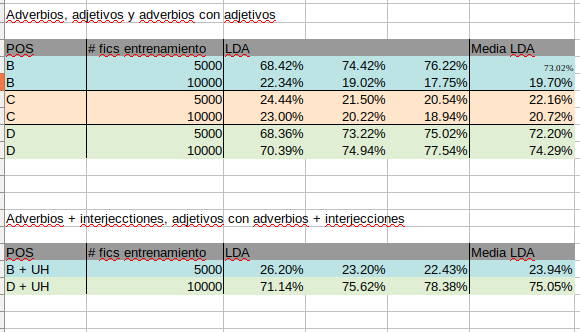
\includegraphics[scale=0.6]{topic_evaluate_table_v2}
	\centering
\end{figure}

Las primeras pruebas mostraron que los modelos B y D eran los que arrojaban mejores resultados. Observando qué otras categorías morfológicas el \textit{tagger} de NLTK puede identificar, pensé que añadir interjecciones a los modelos podría aumentar su precisión. Llamé B+UH y D+UH a los modelos resultantes, y repetí las pruebas. Los resultados están en la segunda tabla de la figura \ref{table:topic_evaluation}.

Curiosamente, el modelo D fue mejorado ligeramente teniendo en cuenta las interjecciones, pero el modelo B empeoró considerablemente.

\section{REFERENCIAS}




\bibliographystyle{alpha}
\singlespacing
\bibliography{ejemplo}


\end{document}


% Local Variables:
% coding: utf-8
% mode: flyspell
% ispell-local-dictionary: "castellano8"
% mode: latex
% End:
